%%%%%%%%%%%%%%%%%%%%%%%VICARIOUS%%%%%%%%%%%%%%%%%%%%%%%%%%%%%%%%%%%%%%%
% FCK CPRGHT												%
% Template for presentation in Latex`s Beamer Class					%
% Using the default Berlin theme, can be replaced by other themes		%
% logo in the upper right can be replaced by new .png, gif, eps etc	%
% 																		%
%%%%%%%%%%%%%%%%%%%%%%%%%%%%%%%%%%%%%%%%%%%%%%%%%%%%%%%%%%%%%%%%%%%%%%%
\documentclass[xcolor=dvipsnames]{beamer}
\usetheme{Berlin}
\usecolortheme[named=LimeGreen]{structure}
\usepackage{beamerthemesplit} % kam neu dazu
\usepackage[ngerman]	{babel}			
\usepackage{t1enc}						
\usepackage[utf8]{inputenc}			
\usepackage{amsmath}
\usepackage{graphicx}
\graphicspath{{pictures/}}
\usepackage{amssymb}
\usepackage{amsfonts}
\usepackage{caption}
\usepackage{multimedia}
\usepackage{tikz}
\usepackage{listings}
\usepackage{acronym}
\usepackage{subfig}

\usepackage{lmodern}
\usepackage{multicol}

\definecolor{pblue}{rgb}{0.13,0.13,1}
\definecolor{pgreen}{rgb}{0,0.5,0}
\definecolor{pred}{rgb}{0.9,0,0}
\definecolor{pgrey}{rgb}{0.46,0.45,0.48}

\lstset{
    escapeinside={(*}{*)}
}

\lstdefinestyle{Java}{
  showspaces=false,
  showtabs=false,
  tabsize=2,
  breaklines=true,
  showstringspaces=false,
  breakatwhitespace=true,
  commentstyle=\color{pgreen},
  keywordstyle=\color{pblue},
  stringstyle=\color{pred},
  basicstyle=\footnotesize\ttfamily,
  numbers=left,
  numberstyle=\tiny\color{gray}\ttfamily,
  numbersep=7pt,
  %moredelim=[il][\textcolor{pgrey}]{$$},
  moredelim=[is][\textcolor{pgrey}]{\%\%}{\%\%},
  captionpos=b
}

\lstdefinestyle{basic}{  
  basicstyle=\footnotesize\ttfamily,
  breaklines=true
  numbers=left,
  numberstyle=\tiny\color{gray}\ttfamily,
  numbersep=7pt,
  backgroundcolor=\color{white},
  showspaces=false,
  showstringspaces=false,
  showtabs=false,
  frame=single,
  rulecolor=\color{black},
  captionpos=b,
  keywordstyle=\color{blue}\bf,
  commentstyle=\color{gray},
  stringstyle=\color{green},
  keywordstyle={[2]\color{red}\bf},
}


\lstdefinelanguage{custom}
{
morekeywords={public, void},
sensitive=false,
morecomment=[l]{//},
morecomment=[s]{/*}{*/},
morestring=[b]",
}


\lstdefinestyle{BashInputStyle}{
  language=bash,
  showstringspaces=false,
  basicstyle=\small\sffamily,
  numbers=left,
  numberstyle=\tiny,
  numbersep=5pt,
  frame=trlb,
  columns=fullflexible,
  backgroundcolor=\color{gray!20},
  linewidth=0.9\linewidth,
  xleftmargin=0.1\linewidth
}

%Logo in the upper right just change if you know what you are doing^^
\addtobeamertemplate{frametitle}{}{%
\begin{tikzpicture}[remember picture,overlay]
\node[anchor=north east,yshift=2pt] at (current page.north east) {
\includegraphics[height=1.8cm]{htw}};
\end{tikzpicture}}

\begin{document}
\bibliographystyle{alpha}
\title{Netzwerke -- Seminaristische Übung WS17/18}
\subtitle{Bit-Arithmetik \& OSI Layer I\\
		\href{mailto:Benjamin.Troester@HTW-Berlin.de}{Benjamin.Troester@HTW-Berlin.de}\\
		PGP: ADE1 3997 3D5D B25D 3F8F 0A51 A03A 3A24 978D D673 }
\author{Benjamin Tröster}

\date{\today}

\begin{frame}
\titlepage

\end{frame}

\section*{Road-Map}
\begin{frame}
\frametitle{Road-Map}
\begin{multicols}{2}
  \tableofcontents
\end{multicols}
\end{frame}

\section*{Stuff}
\begin{frame}{Nerd-Wochenmarkt}
Empfehlung der Woche:
\begin{itemize}
	\item n00bCore:
	\begin{itemize}
		\item \glqq n00bfreundlicher Podcast über Computer\grqq
		\item \url{http://n00bcore.de/nc-006-was-ist-ein-internet/}
	 	\item \url{http://n00bcore.de/nc007-away/} 
	\end{itemize}
\end{itemize}
\end{frame}

\begin{frame}{Retrospektive}
\begin{itemize}
	\item Vorlesung
	\begin{itemize}
		\item Fragen?
	\end{itemize}
	\item Übungsblatt
	\begin{itemize}
		\item Auflösung des letzten Aufgabenblatts
		\item Fragen?
	\end{itemize}
\end{itemize}
\end{frame}

\section{Zahlensysteme}
\subsection{Stellenwertsystem}
\begin{frame}
Dezimalsystem $\rightarrow$ Basis 10\\
Eine Zahl in der Darstellung
$$a_n \dots a_0.a_{-1} \dots a_{-m} = \sum_{i=-m}^{n} a_i \cdot 10^i, \quad a_i \in \{0,1, \dots , 9\} $$
wird als Dezimalzahl bezeichnet.\\
Bsp.: $23.42 = 2 \cdot 10^1 + 3 \cdot 10^0 + 4 \cdot 10^{-1} + 2 \cdot 10^{-2}$ 
\end{frame}

\begin{frame}
\begin{itemize}
	\item Stelle einer Ziffer innerhalb der Zahl gibt an, mit welcher Potenz von 10 zu multiplizieren ist
	\begin{itemize}
	\item $\rightarrow$ deshalb nennt man ein derartiges System \textbf{Stellenwertsystem}
	\end{itemize}
	\item Darstellung von $\mathbb{N,Z,Q,I,R}$ ($\mathbb{C}$ ebenfalls, aber als Ebene)
	\item Rechner: nur begrenzte Darstellung möglich $\rightarrow$ begrenzter Speicher
\end{itemize}
\end{frame}

\subsection{Stellenwert Basis $b$}
\begin{frame}
Allgemein kann eine natürliche Zahl mit Basis b durch
$$ \sum_{i=-m}^{n} a_i \cdot b^i, \quad a_i \in \{0,1,2, \dots, b-1 \} $$
dargestellt werden
\end{frame}


\subsection{Dualzahlen}
\begin{frame}
\begin{itemize}
	\item Dual (lat. dualis \glqq zwei enthaltend\grqq) $\rightarrow$ Basis 2
	\item Ziffern nur aus den Werten 0 und 1
	\item In der Informatik als Bit, in der E-Technik \glqq on/off\grqq
	\item $ \sum_{i=0}^{n} a_i \cdot b^i, \quad a_i \in \{0,1\}, b = 2  $
	\item Bsp.: $1101_2 = 1 \cdot 2^3 + 1 \cdot 2^2 + 0 \cdot 2^1 + 1 \cdot 2^0 = 13_{10}$
\end{itemize}
\end{frame}

\subsection{Oktal}
\begin{frame}
\begin{itemize}
	\item Oktal (lat. octo -- acht) $\rightarrow$ Basis 8
	\item Ziffern nur aus den Werten $0 \dots 7$
	\item In der Informatik Permissionsbits
	\item $ \sum_{i=0}^{n} a_i \cdot b^i, \quad a_i \in \{0, \dots 7\}, b = 7  $
	\item Bsp.: $4223_8 = 4 \cdot 8^3 + 2 \cdot 8^2 + 2 \cdot 8^1 + 3 \cdot 8^0 = 2195_{10}$
\end{itemize}
\end{frame}

\subsection{Hexadezimal}
\begin{frame}
\begin{itemize}
	\item Hexadezimal (griech. hexa -- sechs \& lat. decem -- zehn) $\rightarrow$ Basis 16
	\item Ziffern nur aus den Werten $0, \dots 9$ und Zeichen $A, \dots, F$ 
	\item In der Informatik Codierung von MAC-Adressen, Farbwerten, ...
	\item $ \sum_{i=0}^{n} a_i \cdot b^i, \quad a_i \in \{0, \dots 9, A, \dots, F \}, b = 16  $
	\item Bsp.: $1310_{16} = 1 \cdot 16^3 + 3 \cdot 16^2 + 1 \cdot 16^1 + 0 \cdot 16^0 = 4880_{10}$
\end{itemize}
\end{frame}


\section{Umrechnung von Zahlensysteme}
\subsection{Basis b $\rightarrow$ Dezimal}
\begin{frame}
\begin{itemize}
	\item Ganze Zahlen, 
	\item Zahlen mit Basis b
	\item Allgemeim:
			$$ \sum_{i=-m}^{n} a_i \cdot b^i, \quad a_i \in \{0,1,2, \dots, b-1 \} $$
		\item Horner-Schema
	\item Das Polynom $p(x) = b_0 + b_1 x + b_2 x^2 + \dots + b_n x^n$ vom Grad $n$ kann mithilfe des Horner-Schemas durch $p(x) = (\dots (b_n x + b_{n-1})x + \dots) x + b_0$ definiert werden.

\end{itemize}
\end{frame}

\subsection{Dezimal $\rightarrow$ Basis b}
\begin{frame}
\begin{itemize}
	\item Divisionsmethode (Restverfahren)
	\item Konvertierung ganzer Zahlen: 
	\begin{itemize}
		\item Die Zahl wird solange durch die Zahlensystem-Basis geteilt bis die ganzzahlige Teilung das Ergebnis 0 liefert
		\item  Bei jedem Schritt wird der Rest notiert
		\item Rest-Ziffern liefern die Zahl im anderen Zahlensystem
	\end{itemize}
\end{itemize}	
\end{frame}

\begin{frame}
\begin{itemize}
 \item $6172{10} \rightarrow 1100000011100_2$ 
 \begin{table}
\begin{tabular}{lllc} 
Dividend & Divisor & Quotient & Rest\\
6172 & 2 & 3086 & 0 \\
3086 & 2 & 1543 & 0 \\
1543 & 2 & 771 & 1 \\
771 & 2 & 385 & 1 \\
385 & 2 & 192 & 1 \\
192 & 2 & 96 & 0 \\
96 & 2 & 48 & 0 \\
48 & 2 & 14 & 0 \\
24 & 2 & 12 & 0 \\
12 & 2 & 6 & 0 \\
6 & 2 & 3 & 0 \\
3 & 2 & 1 & 1 \\
1 & 2 & 0 & 1 
\end{tabular}
 \end{table}
\end{itemize}
\end{frame}

\section{Bit-Arithmetik}
\subsection{Bit-Wertigkeit}
\begin{frame}
\begin{itemize}
	\item Legt den Stellenwert der Bits fest
	\item Legt das Vorzeichen fest -- Vorzeichenbit
	\item LSB-0-Bitnummerierung -- least significant bit
	\begin{itemize}
		\item Bit am Index 0 niedrigsten Stellenwert
		\item $\sum_{i=0}^{n-1} a_i \cdot 2^i$
		\item Stellen gemäß ihrer absteigenden Wertigkeit -- rechts beginnend
	\end{itemize}
	\item MSB-0-Bitnummerierung -- most significant bit
	\begin{itemize}
		\item Bit am Index 0 höchsten Stellenwert
		\item $\sum_{i=0}^{n-1} a_i \cdot 2^{n-1-i}$
		\item Stellen gemäß ihrer absteigenden Wertigkeit -- links beginnend
	\end{itemize}
\end{itemize}
\end{frame}

\subsection{Byte-Wertigkeit}
\begin{frame}
\begin{itemize}
	\item Bitnummerierung ist unabhängig von der Byte-Reihenfolge 
	\item Werden je acht Bits zu einem Byte gruppiert und diese wiederum zu größeren Zahlenformaten, so ist zusätzlich die Byte-Reihenfolge wichtig
	\item Big- / Little-Endian-Architektur
\end{itemize}
\end{frame}

\subsection{Umrechnung Bit $\leftrightarrow$ Byte ...}
\begin{frame}
\begin{itemize}
	\item Zusammenfassung von 8 Bit zu einem Byte
	\item Speicherkapazitäten mit Zweierpotenz $2^n$-Byte
	\item $2^{10} = 1024$ statt 1000
	\item 1 Kilobyte (kB) = 1000 Byte, 1 Megabyte (MB) = 1000 Kilobyte = 1000 $\cdot$ 1000 Byte = 1.000.000 Byte
	\item IEC-Präfixe:
	\begin{itemize}
		\item 1 Kibibyte (KiB) = 1024 Byte, 1 Mebibyte (MiB) = 1024 $\cdot$ 1024 Byte = 1.048.576 Byte.
	\end{itemize}
\end{itemize}
\end{frame}

\begin{frame}
\begin{figure}
\centering
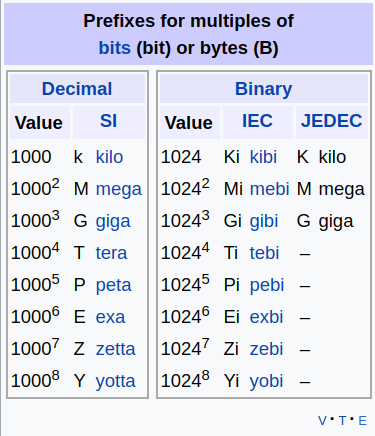
\includegraphics[scale=0.54]{bit-byte}
\end{figure}
\end{frame}

\section{Netzwerkgeräte}
\begin{frame}
\begin{figure}%
    \centering
    \subfloat{{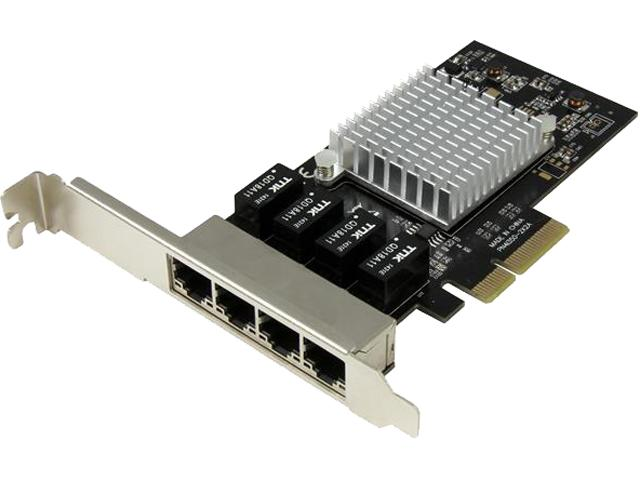
\includegraphics[width=4.5cm]{nw_card1} }}%
    \qquad
    \subfloat{{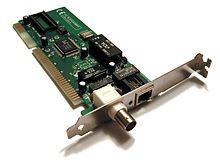
\includegraphics[width=4.5cm]{nw_card2} }}%
\end{figure}
\end{frame}

\begin{frame}
\begin{figure}%
    \centering
    \subfloat{{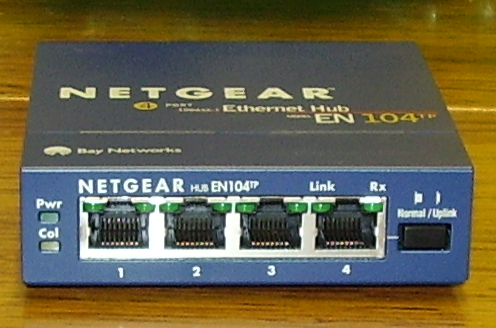
\includegraphics[width=4.5cm]{hub} }}%
    \qquad
    \subfloat{{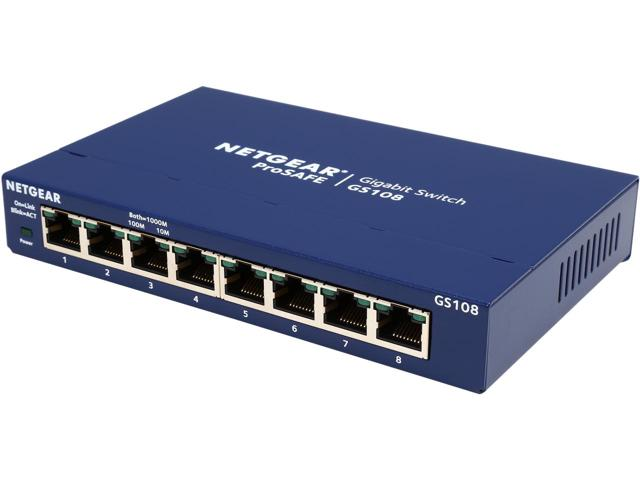
\includegraphics[width=4.5cm]{switch} }}%
\end{figure}
\end{frame}

\begin{frame}
\begin{figure}%
    \centering
    \subfloat{{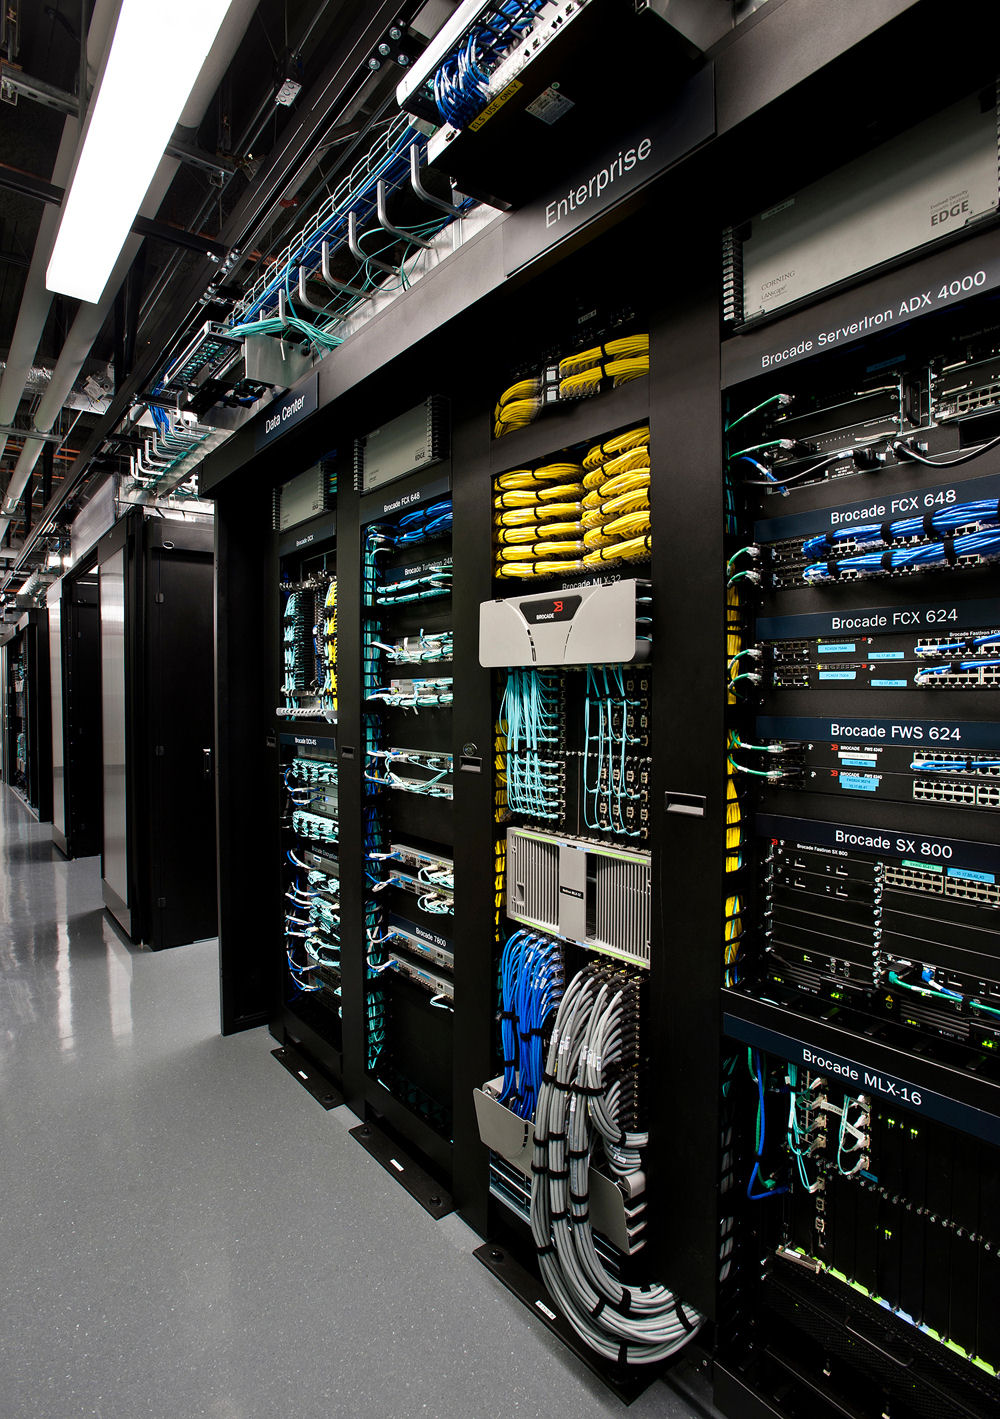
\includegraphics[width=4.5cm]{router} }}%
    \qquad
    \subfloat{{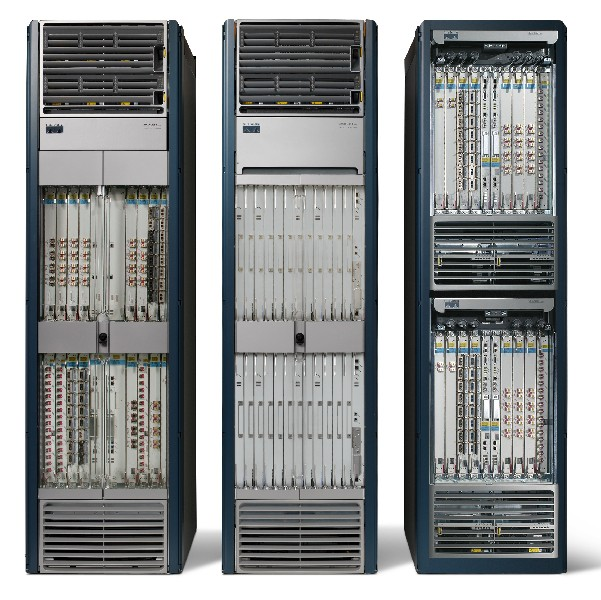
\includegraphics[width=4.5cm]{core_router} }}%
\end{figure}
\end{frame}



\end{document}